\section{Physikalische Grundlagen}

\subsection{Das Prinzip des Lasers}
Der Begriff des Lasers (Light Amplification by stimulated Emission of Radiation) geht bis auf die  Physiker Schawalow und Townes im Jahre  1958 zurück. Diese stellten Überlegungen an, wie man den bis dahin  bekannten Maser (microwave amplification) auf den optischen Spektralbereich ausdehnen könnte. Heutzutage ist der Laser ein in der  Wissenschaft nicht mehr wegzudenkendes Instrument der Initiierung,  Messung und Steuerung komplexer Prozesse.

\subsection{Emission und Absorption}
Die Elektronen von Atomen befinden sich im Grundzustand alle im energetisch günstigsten Zustand $E_!$. Durch  Energiezufuhr können diese  in energetisch höhere Zustände $E_2$ angeregt werden. Dabei muss die zugeführte Energie genau der Energiedifferenz zwischen den Zuständen entsprechen: $E_2 = E_1 +h\nu$.Man spricht  von gequantelter Absorption. Umgekehrt kann ein Elektron aus einem höheren Zustand durch  Abgabe von Energie in einen unbesetzten niedrigeren Zustand übergehen.  Dabei wird  dann entsprechend  ein Photon mit der Übergangsenergie emittiert.

\subsection{Die Einsteinkoeffizienten}
Albert Einstein führte 1916 drei Koeffizienten zur Beschreibung der Emission und der Absorption ein:

\begin{tabular}{l l}
$B_{12}$ & Beschreibt die Absorption, also die Anregung des Atoms durch ein Photon der Energie $h\nu$ \\
& in einen energetisch höheren Zustand.\\
$B_{21}$ & Beschreibt die stimulierte Emission. Hierbei befindet sich das Atom in einem angeregten Zustand. \\
& Durch eintreffen eines Photons wird eine Relaxion in das niedriger Niveau bewirkt. Durch diesen\\
&  Übergang wird ein Photon erzeugt, welches die selbe Energie wie das eintreffende hat.\\
$A_{21}$ & beschreibt die spontane Emission: Das angeregte Atom relaxiert dabei spontan in ein niedrigeres\\
& Energieniveau, wobei wieder  ein Photon emittiert wird.
\end{tabular}

Über diese Koeffizienten kann nun Berechnet werden, wie viele Atome pro Zeit in einem Strahlungsfeld der Energiedichte $\omega_{\nu}$,  durch Absorption in einen höheren Zustand übergehen:

\begin{equation}
\frac{dN_1}{dt}=-N_1 \cdot B_{12} \cdot \omega_{\nu} + N_2 \cdot B_{21} \cdot \omega_{\nu} + N_2 \cdot A_{21}
\end{equation}

Die Übergangsrate des umgekehrten Übergangs (unter Emission eines Photons) ergibt sich genau umgekehrt:

\begin{equation}
\frac{dN_1}{dt}= N_1 \cdot B_{12} \cdot \omega_{\nu} - N_2 \cdot B_{21} \cdot \omega_{\nu} - N_2 \cdot A_{21}
\end{equation}

Im thermodynamischen Gleichgewicht ist  die Absorption gleich der Emission,sodass die Besetzungszahlen der Zustände der Boltzmann-Verteilung folgen. Da unsere Zustände entartet sein können, muss dies als zusätzliche Gewichtung $g=(2J+1)$ in die Verteilung mit einfließen:

\begin{equation}
\frac{N_1}{N_2} = \frac{g_1}{g_2} e^{-h\nu/k_BT}
\end{equation}

Setzt man nun beide Übergangsraten gleich, erhält man:

\begin{align}
\frac{dN_1}{dt} =& \frac{dN_2}{dt}\\
\leftrightarrow \frac{N_1}{N_2} =& \frac{B_{21}\cdot \omega_{\nu} +A_{21}}{B_{21}\cdot \omega_{\nu}} = \frac{g_1}{g_2}e^{\frac{h\nu}{k_BT}} \\
\leftrightarrow \omega_{\nu}(\nu) =& \frac{A_{21}/B_{21}}{(g_1/g_2)(B_{12}/B_{21})\cdot e^{h\nu/kT}-1}
\end{align}

Diese Formel für die spektrale Energiedichte kann man mit der Planckschen Strahlungsformel für die Energiedichte vergleichen:

\begin{equation}
\omega_{\nu}(v) = \frac{8\pi h\nu^3}{c^3}\frac{1}{e^{h\nu/k_B T}-1}
\end{equation}

Aus dieser erhält man die Beziehung für die Einsteinkoeffizienten:

\begin{align}
B_{12} &= \frac{g_2}{g_1}B_{21}\\
A_{21} &= \frac{8\pi h\nu^3}{c^3}B_{21}
\end{align}

Da das Verhältnis von $A_{21}$ zu $B_21$ proportional zu $\nu^3$ ist, sind Laser mit sehr kurzen Wellenlängen schwer zu realisieren.

\subsection{Der Grundaufbau}

Ein Laser besteht grundsätzlich aus drei Komponenten:
\begin{enumerate}
\item einem aktiven Medium
\item einer Energiepumpe
\item einem optischen Resonator
\end{enumerate}

\begin{figure}[here]
\centering
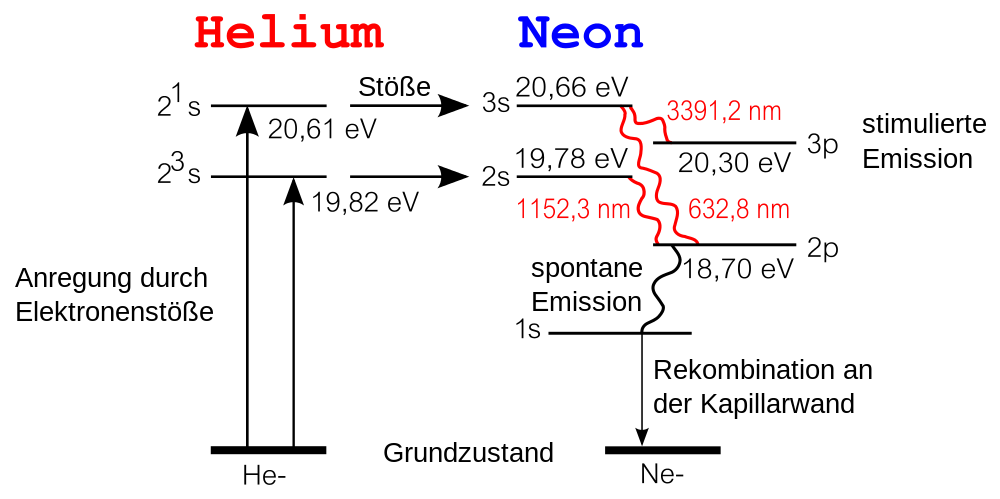
\includegraphics[scale=0.4]{HNL2.png}
\begin{center}
\end{center}
\end{figure}
